%==============================================================================
%  SEP 740 -- Article-Style Project Report (IEEE conference format)
%
%  Limit: 5 pages of content, a 6th page permitted for references only.
%  No table of contents and no abstract, by instruction.
%
%  Compile with:  pdflatex ieee_paper.tex   (run twice for cross-references)
%  Requires:      figures/ieee_*.png, regenerated by
%                 python paper_experiments.py --figures
%==============================================================================
\documentclass[conference]{IEEEtran}
\IEEEoverridecommandlockouts

\usepackage{cite}
\usepackage{amsmath,amssymb}
\usepackage{graphicx}
\usepackage{booktabs}
\usepackage{balance}
\usepackage[hidelinks]{hyperref}

\graphicspath{{figures/}}

% -----------------------------------------------------------------------------
% Page numbers. IEEEtran's conference mode suppresses them, because IEEE
% paginates proceedings itself. Enabled here only so the page limit can be
% checked during marking. Delete this block for an actual IEEE submission.
% -----------------------------------------------------------------------------
\usepackage{fancyhdr}
\fancypagestyle{numbered}{%
  \fancyhf{}%
  \fancyfoot[C]{\thepage}%
  \renewcommand{\headrulewidth}{0pt}%
  \renewcommand{\footrulewidth}{0pt}%
}
\pagestyle{numbered}

\begin{document}

\title{Facial Recognition Using OpenFace Inception Network}

% NOTE: the fifth surname was truncated in the source roster ("Yaathaven
% Sathanan..."); complete it before submitting. Author order is the roster order,
% not a contribution ordering -- reorder if the group agrees otherwise.
\author{\IEEEauthorblockN{Arne Tirez, Gurtaj Singh, Jenil Bhayani,
                          Mike Zhang, and Yaathaven Sathananthan}
\IEEEauthorblockA{\textit{SEP 740 -- Deep Learning}\\
\textit{McMaster University}, Hamilton, ON, Canada}}

\maketitle
\thispagestyle{numbered}   % IEEEtran forces page 1 to \pagestyle{empty}

%==============================================================================
\section{Introduction}
%==============================================================================

A facial recognition model can perform several different tasks depending on the application. Verification is a one-to-one problem in which the model acts as a binary classifier, determining whether an input face matches a specific claimed identity. Closed-set identification is a one-to-N problem in which the model compares an input photo against N enrolled people in its database and identifies the correct person, assuming the individual is already enrolled. Open-set identification is similar to closed-set identification, but it also allows the model to determine that the input face does not belong to anyone in the database and classify it as an unknown or unidentifiable person.~\cite{klare2015ijba}.

Many published facial recognition models were developed and evaluated for verification rather than identification. For example, OpenFace reported an accuracy of
$92.92\% \pm 1.34\%$, and FaceNet reported an accuracy of  $99.63\%$, with both models evaluated on the standard LFW dataset, which is designed for verification tasks.
The same is true for DeepFace~\cite{taigman2014deepface} and most models on the LFW leaderboard.

We built a model on the pretrained OpenFace \texttt{nn4.small2}
network~\cite{amos2016openface} and evaluate all three tasks on Labeled Faces in
the Wild (LFW)~\cite{huang2007lfw} using identical embeddings. On the same
embedding we measure $89.2\%$ verification, $58.7\%$ closed-set rank-1 on a
$150$-identity gallery, and $14.7\%$ open-set detection and identification rate at
$1\%$ false accept rate.

Our contributions are:

\begin{enumerate}
\item A comparison of verification, closed-set identification, and open-set identification using the same face embedding, furthermore the preprocessing will be tuned on a separate validation dataset to ensure the reported accuracy is unbiased.

\item This assignment also explains the performance gap in closed-set identification using an order-statistics model. The facial recognition model was first evaluated on a test dataset to obtain its actual identification accuracy. The per test image and pooled approaches were then used to predict that accuracy, and their predictions were compared with the measured results. The per test image approach closely matched the actual performance, whereas the pooled approach was much less accurate. The remaining differences indicated that the assumption that each face comparison was independent did not always hold in practice.

\item Two preprocessing steps were tested to see how it affected performance. On the tuning dataset, using a smaller face crop improved accuracy by 17.1\%. Furthermore, moving the crop window 18 pixels downward improved the accuracy by 12.7–14.6\%  while keeping the crop size the same.

\item Using multiple reference photos for each person improved the model's identification accuracy from 52.0\% to 69.3\%. It can also be confirmed that this improvement was due to the proposed method, rather than face embeddings becoming more similar.

\end{enumerate}

All reported numbers and figures are produced by
paper\_experiments.py in the accompanying
repository,\footnote{\url{https://github.com/fistfulofyen/Face_sys_LFW}} which is
seeded throughout and prints each result under the table it feeds. The one
exception is the detector comparison of Section~\ref{sec:detector}, which requires
an external model file not redistributed with the repository.

%==============================================================================
\section{Background}
%==============================================================================

\subsection{Metric Learning}

A softmax classifier has one output for each identity. Whenever a new identity is added to the database, the model must be retrained, and thus output layer will grow. It also cannot identify someone as "unknown" because it can only choose from the identities stored.

Deep metric learning instead learns an embedding
$f:\mathcal{I}\rightarrow\mathbb{R}^{128}$ in which Euclidean distance encodes
identity.To add a new person, the model only needs to process their reference photo once. It can also recognize when a face does not match anyone in the database by using a similarity threshold.

\subsection{Triplet Loss}

FaceNet~\cite{schroff2015facenet} trains the model using three images at a time: an anchor image
$A$, a positive image of the same person $P$,and a negative image of a different person $N^-$. The model learns to make the anchor and positive images closer together than the anchor and negative images by at least a margin $\alpha$:
\[
\|f(A)-f(P)\|_2^2 + \alpha \le \|f(A)-f(N^-)\|_2^2.
\]

The triplet loss used during training is:

\begin{equation}
\mathcal{L}=\sum_i \max\!\big(\lVert f(A_i)-f(P_i)\rVert_2^2
 -\lVert f(A_i)-f(N^-_i)\rVert_2^2+\alpha,\;0\big).
\end{equation}

The margin $\alpha$ is essential because it forces the model to separate images of different people. Since the number of possible triplets grows cubically in the training set size, training uses semi-hard negatives:
\
$\lVert f(A)-f(P)\rVert_2^2 < \lVert f(A)-f(N^-)\rVert_2^2 <
 \lVert f(A)-f(P)\rVert_2^2+\alpha$
 \
 
Later work replaces sampled triplets with angular margins such as, CosFace~\cite{wang2018cosface} and ArcFace~\cite{deng2019arcface}.

\subsection{Embedding Normalization and Distance Metrics}

$L^2$ normalisation places embeddings on the unit hypersphere, so distances are
bounded to $[0,2]$ rather than $[0,1]$, and
$\lVert f(x_i)-f(x_j)\rVert_2^2 = 2-2\cos\theta_{ij}$ makes squared Euclidean
distance and cosine similarity interchangeable for ranking.

\textbf{All distances and thresholds here are unsquared $L^2$.} This matters
because OpenFace's own default threshold of $0.99$ is on $L^2$,
equivalent to $0.995$ unsquared. Although this value is close to the threshold found in this study, the similarity is only due to the dataset and does not mean the same threshold was rediscovered. Using the $L^2$ distance, the threshold found in this study would be $0.984$.

%==============================================================================
\section{Method}
%==============================================================================

\subsection{Model}

The model is an Inception-style CNN~\cite{szegedy2015going} with $3{,}733{,}968$
trainable parameters over $155$ layers, comprising $37$ convolutions, $37$
batch-normalization layers, and $7$ depth concatenations. Keras reports a total of $3{,}743{,}280$ parameters, with the extra $9{,}312$ parameters coming from the non-trainable moving means and variances used in the batch-normalization layers. The number of trainable parameters matches the value reported by OpenFace, confirming that the implementation is accurate.

It maps a channels-first $(3,96,96)$ RGB tensor to a $128$-dimensional unit-norm
vector. A three-block stem downsamples the image to $12\times12$. Seven Inception stages then
reduce it further to $3\times3$ while increasing the  depth to $736$ channels. Finally a dense layer with $L^2$ normalisation produces the face embedding. The $1\times1$ branches inside
each stage act as bottlenecks to hold the parameter count at $3.7$M.

The network is a frozen feature extractor with pretrained OpenFace weights. These weights were orginally trained on CASIA-WebFace and FaceScrub datasets containing about, $500{,}000$ face images. This is about $400\times$ less data than the private dataset used to train FaceNet, therefore the appropriate baseline for this reproduction is OpenFace's $92.92\% \pm 1.34\%$, not FaceNet's $99.63\%$.

\subsection{Model Weight Implementation}

The model parameters were provided as $226$ CSV files exported from the original Torch model, of which $224$ are used: two tensors for each of $37$ convolutions, four for each of $37$
batch-normalisation layers, and two for the dense layer. The two unused files are
the moving mean and variance exported for inception\_5a\_3x3\_conv2, a
convolution that has no batch-normalisation layer in this architecture. To load the weights correctly requires
transposing convolution kernels from Torch's $(\text{out},\text{in},h,w)$ layout to
TensorFlow's $(h,w,\text{in},\text{out})$. One important detail from the original model was also preserved:
the first stem block uses $\varepsilon=10^{-3}$, while all $36$ others use
$10^{-5}$. Our implementation reproduces the embeddings of the Keras-OpenFace
reference port to $0.000\mathrm{e}{+}00$ maximum element-wise difference, with all
$75$ weight-bearing layers matching.

\subsection{Identification and Verification Methods}

The classifier is non-parametric, meaning it does not need to be retrained when new people are added. For verification, a face is accepted if
\
$\lVert f(x)-e_{\text{claim}}\rVert_2 < \tau$
\
For closed-set identification, the model returns the identity with the smallest distance:
\
$\arg\min_k \lVert f(x)-e_k\rVert_2$
\
Open-set identification returns that
argument only if the corresponding minimum falls below $\tau$, and otherwise
it classifies the face as unknown. Following~\cite{klare2015ijba}, open-set performance is measured using the Detection and Identification Rate (DIR), which is the percentage of people with reference photos in the database who are both correctly identified and accepted.

%==============================================================================
\section{Experimental Setup}
%==============================================================================

LFW contains $13{,}233$ photographs of $5{,}749$ individuals from online news
sources. We use the \texttt{lfw-deepfunneled} version, where the faces have already been aligned. Of its
identities $70.8\%$ have exactly one photograph; these can populate the mismatched
half of the pairs list and serve as open-set unknown probes, but cannot be
closed-set probes.

To avoid selection bias, this project seperates the official LFW pairs into two independent sets: a 600-pair tuning set and a 600-pair test set. The tuning set was used to choose the best crop settings, while the test set was used only for the final evaluation. Although the two sets contain different image pairs, 99 individual images appear in both because some LFW images are reused in multiple pairs.

A limitation of the study is that the crop settings were chosen before the tuning and test sets were created, so they may have been influenced by some of the test data. To reduce this bias, we repeated the crop experiments on the tuning set and confirmed that the chosen crop performed nearly as well as the best possible setting. We kept the original crop settings and acknowledged that a small amount of bias may still remain.


We use $600$ of the $3{,}000$ available pairs per half to keep the
nine-configuration ablation practical to run on CPU. This caused us to have wider confidence intervals due to fewer image pairs, which translates into the results being less precise. We acknowledge that if all 3,000 pairs were included then it would have produced more precise estimates.

Three quantities appear in the literature as ``accuracy.'' Cross-validation (CV) accuracy finds the best threshold $\tau$ using ten-fold cross-validation. Fixed-threshold accuracy measures performance using one chosen threshold. Best-threshold accuracy reports the highest accuracy obtained by testing many thresholds on the same data, which can produce optimistic results. Unless otherwise stated, all reported accuracies are CV accuracies. Unlike the original LFW protocol, the authors created random folds from their own 600-pair sample instead of using LFW's predefined identity-disjoint folds.

We selected $300$ people with multiple photos. Each person was represented by one reference photo in the database, while a second photo was used as the probe image. For each database size (N), the results were averaged over $200$ randomly generated databases so that every experiment was evaluated consistently. The only exception was $(N = 300)$, where only one possible database existed.

%==============================================================================
\section{Explanation of the Source Code}
%==============================================================================

The implementation consists of two modules, one script, and one notebook.
\texttt{facenet\_arch.py} (280 lines) builds the network from two helper functions,
one for a convolutional branch and one for a pooling branch, so each Inception
stage is written as a short list of branches. The \texttt{name} given to each
weight-bearing layer is functional rather than cosmetic, since those strings are
the keys used to match a layer to its weight file.
\texttt{facenet\_utils.py} (523 lines) reads the CSV weight exports and converts
them from Torch to TensorFlow layout, loads and crops images, builds the identity
database, and provides the evaluation helpers.
\texttt{paper\_experiments.py} (392 lines) runs the five reported experiments and
is seeded, so re-running it reproduces the values given here.
\texttt{face\_recognition\_pipeline.ipynb} (38 code cells) is a walkthrough version
for reading, not the source of the reported results.

%==============================================================================
\section{Results}
%==============================================================================

\subsection{Preprocessing}
\label{sec:prep}

\begin{table}[!t]
\caption{Effect of crop size and crop position on ten-fold cross-validation accuracy for the tuning and test datasets.}
\label{tab:crop}
\centering
\begin{tabular}{lcc}
\toprule
Crop window & Tuning split & Test split \\
\midrule
None (full $250$ px frame) & 57.7\% & 56.8\% \\
$160$ px, centred          & 64.5\% & 66.8\% \\
$128$ px, centred          & 66.2\% & 65.8\% \\
$110$ px, centred          & 72.0\% & 72.2\% \\
$96$ px, centred           & 74.8\% & 74.3\% \\
$92$ px, centred           & 73.7\% & 73.2\% \\
$96$ px, $18$ px lower     & 87.5\% & 89.7\% \\
$\mathbf{92}$ \textbf{px,} $\mathbf{18}$ \textbf{px lower} & \textbf{88.3\%} & \textbf{89.2\%} \\
$88$ px, $18$ px lower     & 88.7\% & 88.8\% \\
\bottomrule
\end{tabular}
\end{table}

Table~\ref{tab:crop} shows the effect of two preprocessing changes evaluated on the tuning set. Reducing the crop window from the full image to 96 × 96 pixels improved accuracy by 17.1\%. Making the crop even smaller to 92 × 92 pixels slightly reduced accuracy, which can be allocated to be measurement noise.

The second preprocessing effect was evaluated while keeping the crop window size fixed so that only its position changed. Moving the crop window 18 pixels downward improved accuracy by 12.7\% for the 96 × 96 window and 14.6\% for the 92 × 92 window. This shows that the position of the crop window has almost as much impact on accuracy as its size. If only the crop size had been optimized, the best accuracy would have been 74.8%.

The explanation is that a centered crop on the deepfunneled LFW images includes more of the forehead and hairline, while the pretrained OpenFace model was trained on crops centered closer to the eyes, nose, and mouth. Shifting the crop downward better matches the data used to train the model. Within the shifted crop windows, changing the crop size had very little effect. This indicates that no crop size was consistently better, whereas moving the crop window 18 pixels downward consistently produced a clear improvement.

The final model uses the $(92 \times 92)$ crop window shifted 18 pixels downward. When evaluated on the held-out test set, the model achieved 89.2\% ± 3.3\% cross-validation accuracy (535/600 pairs), an AUC of 0.97, an EER of 10.0\%, and a threshold of $(\tau = 0.992)$. This is about 4\% lower than OpenFace's reported $(92.92\% \pm 1.34\%)$. The lower performance can be attributed to the lower input data size. 

A control experiment confirmed that the improvement came from changing the crop position rather than the image resizing method. We repeated the uncropped experiment using nearest-neighbor, bilinear, bicubic, area, and Lanczos interpolation, and the accuracy ranged from 56.8\% to 59.5\%, a difference of only 2.7\%.

\begin{figure*}[!t]
\centering
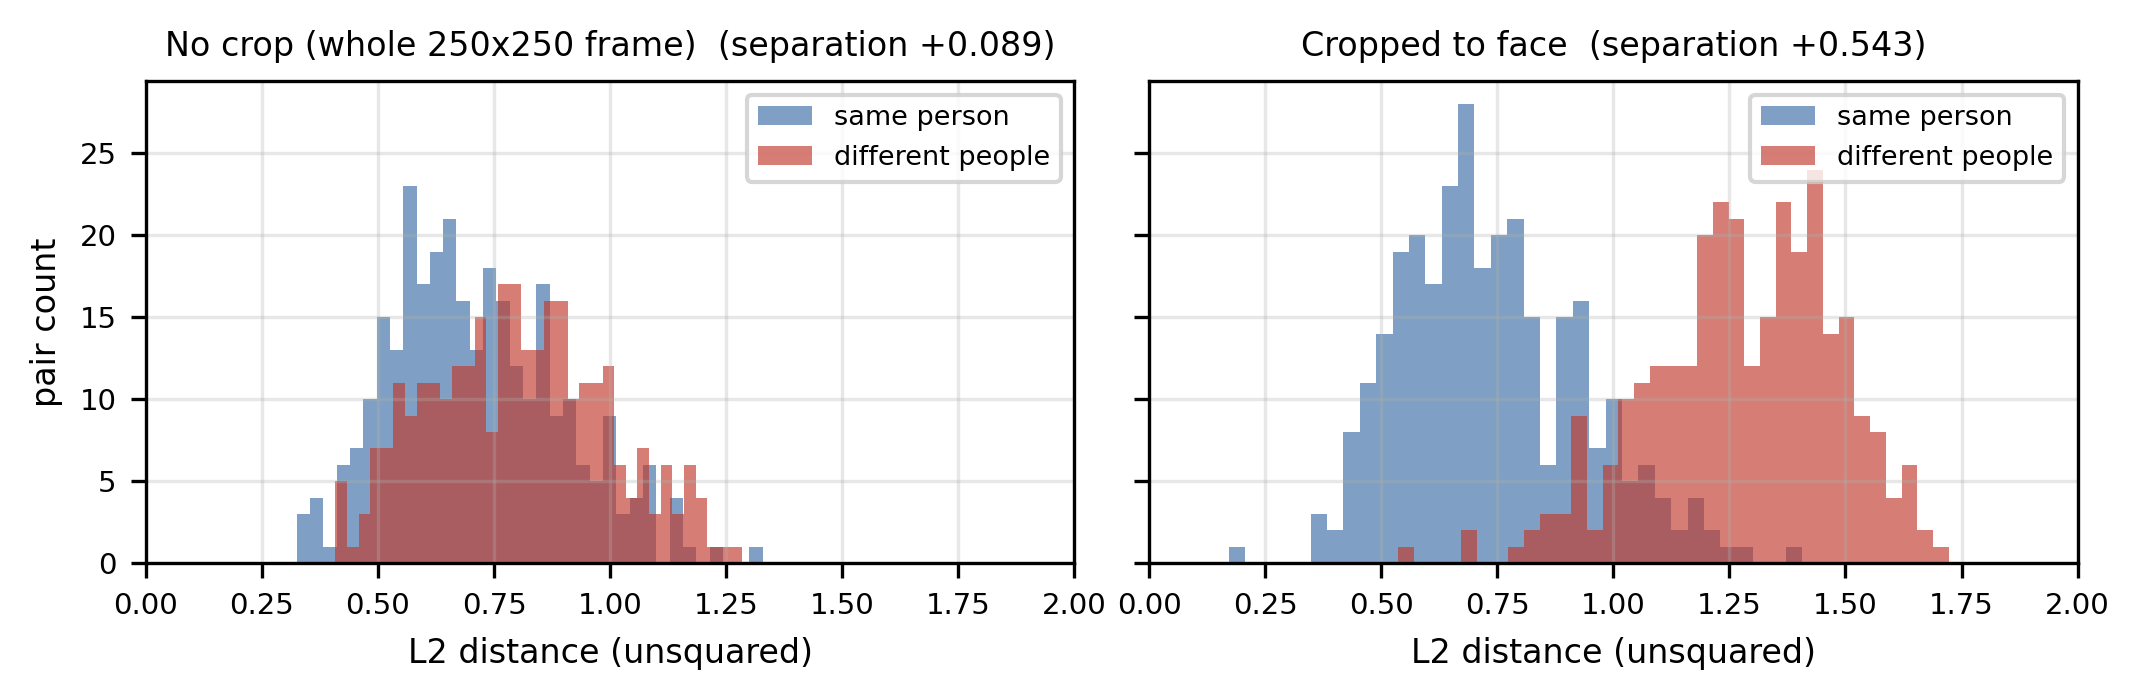
\includegraphics[width=\textwidth]{ieee_distributions.png}
\caption{Matched and mismatched distance distributions on the held-out test split.
         Cropping separates the distributions by roughly a factor of five.}
\label{fig:dist}
\end{figure*}

\subsection{Verification operating points}

\begin{table}[!t]
\caption{Fixed-$\tau$ operating points on the held-out test split.}
\label{tab:operating}
\centering
\begin{tabular}{cccc}
\toprule
Threshold $\tau$ & FAR & FRR & Fixed-$\tau$ accuracy \\
\midrule
0.700 & 1.0\%  & 51.7\% & 73.7\% \\
0.850 & 2.0\%  & 26.7\% & 85.7\% \\
0.950 & 7.0\%  & 14.3\% & 89.3\% \\
\textbf{0.992} (CV-selected) & \textbf{8.3\%} & \textbf{12.0\%} & \textbf{89.8\%} \\
1.100 & 19.7\% & 4.3\%  & 88.0\% \\
1.250 & 42.7\% & 0.7\%  & 78.3\% \\
\midrule
\multicolumn{4}{l}{\emph{Best-$\tau$ accuracy (optimistic, same data): $90.5\%$}} \\
\bottomrule
\end{tabular}
\end{table}

Table~\ref{tab:operating} corrects a common assumption. A threshold of 0.7, which is commonly used in tutorial implementations, is too conservative for this dataset. It incorrectly accepts only 1.0\% of unknown people, but rejects 51.7\% of genuine matches. The best threshold found using cross-validation is close to the equal error rate (EER). Choosing the threshold depends on the application's requirements, and different threshold values can change the accuracy by more than 15\%. The full
operating characteristic is shown in Fig.~\ref{fig:roc}.

\begin{figure}[!t]
\centering
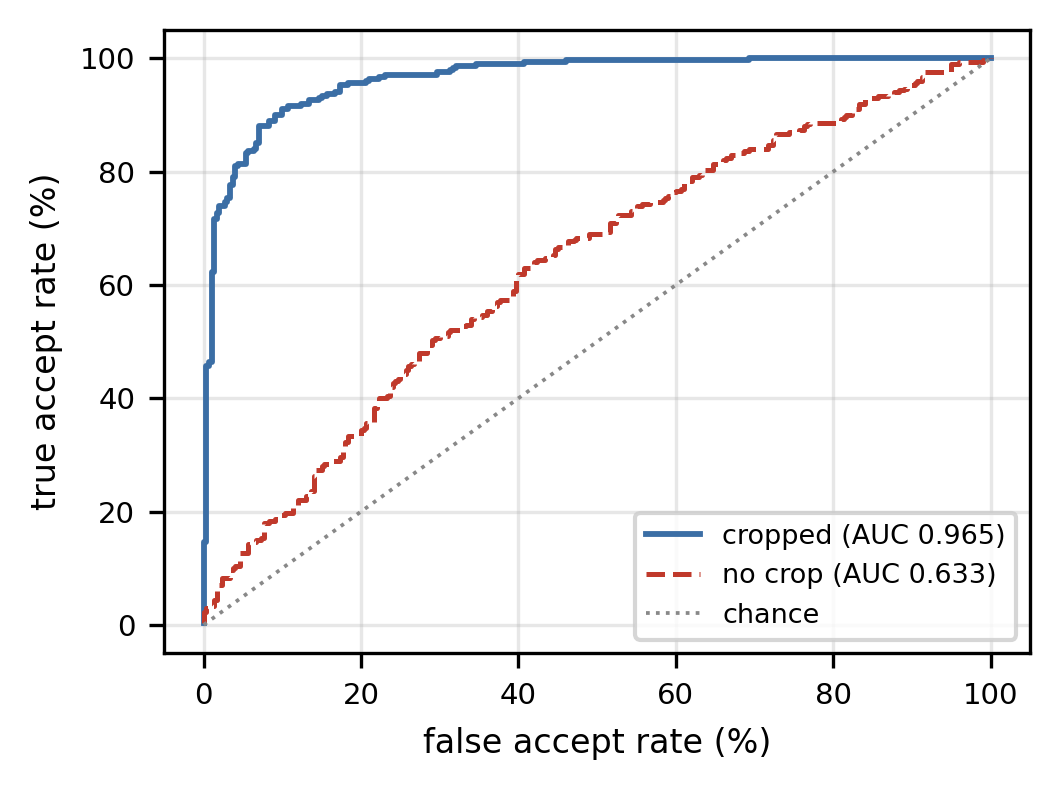
\includegraphics[width=\columnwidth]{ieee_roc.png}
\caption{ROC on the held-out test split, with and without face cropping.}
\label{fig:roc}
\end{figure}

\subsection{Analysis of Closed-Set Identification}
\label{sec:orderstats}

Verification compares a face with one reference photo, while identification compares it with all reference photos in the database. As the number of people in the database increases, the chance that an incorrect person has a very similar face also increases, making identification more difficult. Although the average distance to an incorrect person stays at 1.28, the distance to the closest incorrect match decreases from 1.28 at $(N = 2)$ to 0.70 at $(N = 300)$ (Table III). This is why identification accuracy decreases as the database grows.

Let $p_i$ be the probability that a randomly chosen wrong identity is closer than the correct reference photo. Assuming each incorrect comparison is independent, the per test image prediction is

\begin{equation}
\hat{r}_{\text{probe}}(N) = \frac{1}{n}\sum_{i=1}^{n} (1-p_i)^{N-1},
\label{eq:probe}
\end{equation}
while the pooled prediction is
\begin{equation}
\hat{r}_{\text{pool}}(N) = (1-\bar{p})^{N-1},
\label{eq:pool}
\end{equation}

where $\bar{p}$ is the mean of $p_i$. The two differ only in whether the average
precedes or follows exponentiation.

\begin{table}[!t]
\caption{Observed closed-set identification accuracy compared with the per-test-image and pooled order-statistics predictions for different database sizes.}
\label{tab:orderstats}
\centering
\begin{tabular}{crrrr}
\toprule
$N$ & $\mathbb{E}[\min d_{\text{imp}}]$ & Observed & Eq.~(\ref{eq:probe}) & Eq.~(\ref{eq:pool}) \\
\midrule
2   & 1.28 & $98.3 \pm 9.2$\%  & 96.9\% & 96.9\% \\
5   & 1.07 & $91.3 \pm 13.4$\% & 90.9\% & 88.3\% \\
10  & 0.99 & $85.0 \pm 10.7$\% & 85.0\% & 75.5\% \\
25  & 0.88 & $75.2 \pm 8.7$\%  & 75.8\% & 47.3\% \\
50  & 0.82 & $67.2 \pm 6.1$\%  & 68.5\% & 21.7\% \\
100 & 0.77 & $59.1 \pm 4.4$\%  & 61.3\% & 4.6\% \\
150 & 0.75 & $54.7 \pm 3.1$\%  & 57.5\% & 1.0\% \\
300 & 0.70 & 46.7\%            & 51.9\% & 0.01\% \\
\bottomrule
\end{tabular}
\end{table}

Table~\ref{tab:orderstats} reports $54.7\%$ at
$N=150$ while the headline figure is $58.7\%$.The headline is the accuracy of single database of 150 people, which is the value produced by the released code. The value in Table III is the average accuracy over 200 randomly generated databases of the same size, making it a more reliable estimate because it reduces the effect of any one randomly selected database. The 4.0 percentage point difference is close to the ±3.1 percentage point standard deviation across the 200 databases, showing that a single randomly selected database can easily produce an accuracy several percentages above or below the average.

Eq.~(\ref{eq:probe}) tracks measurement to within $2.8$\% up to $N=150$;
Eq.~(\ref{eq:pool}) is wrong by a factor of $55$ and by three orders of
magnitude for $N=300$.

The $p_i$ are computed from the same $300 \times 300$ distance matrix that was used to evaluate the different database sizes.
As a result Eq.~(\ref{eq:probe}) has no free parameters and no
unseen data.Instead of focusing on how closely the equation matches the results, we examine the remaining errors to determine whether the assumption that all incorrect comparisons are independent is valid. The standard error for a single database size is about 4\% at (N = 150), so individual results should not be overinterpreted. The errors also followed a clear pattern rather than occurring randomly. Eq. (2) underestimated accuracy at (N = 2) and (N = 5), matched the results at (N = 10), and increasingly overestimated accuracy from (N = 25) onward. This pattern suggests that incorrect comparisons are not completely independent, a phenomenon known as hubness~\cite{radovanovic2010hubs}. Therefore, Eq. (2) provides a good approximation but is not an exact model.

Eq.~(\ref{eq:pool}) fails because $\bar{p}=3.1\%$ does not accurately represent any individual test image. The
distribution is bimodal: $140$ of $300$ test images have $p_i$ exactly zero, $111$ fall
in $(0, 0.05)$ and $49$ exceed $0.05$. At (N = 150), the test images with $p_i = 0$ contributed 46.7\% of the total 54.7\% average accuracy, while most of the remaining accuracy came from the images with very small non-zero $p_i$ values. Averaging these probabilities into a single value $\bar{p}$ removes this important structure, which explains why Eq. (3) gives much less accurate predictions

\begin{figure*}[!t]
\centering
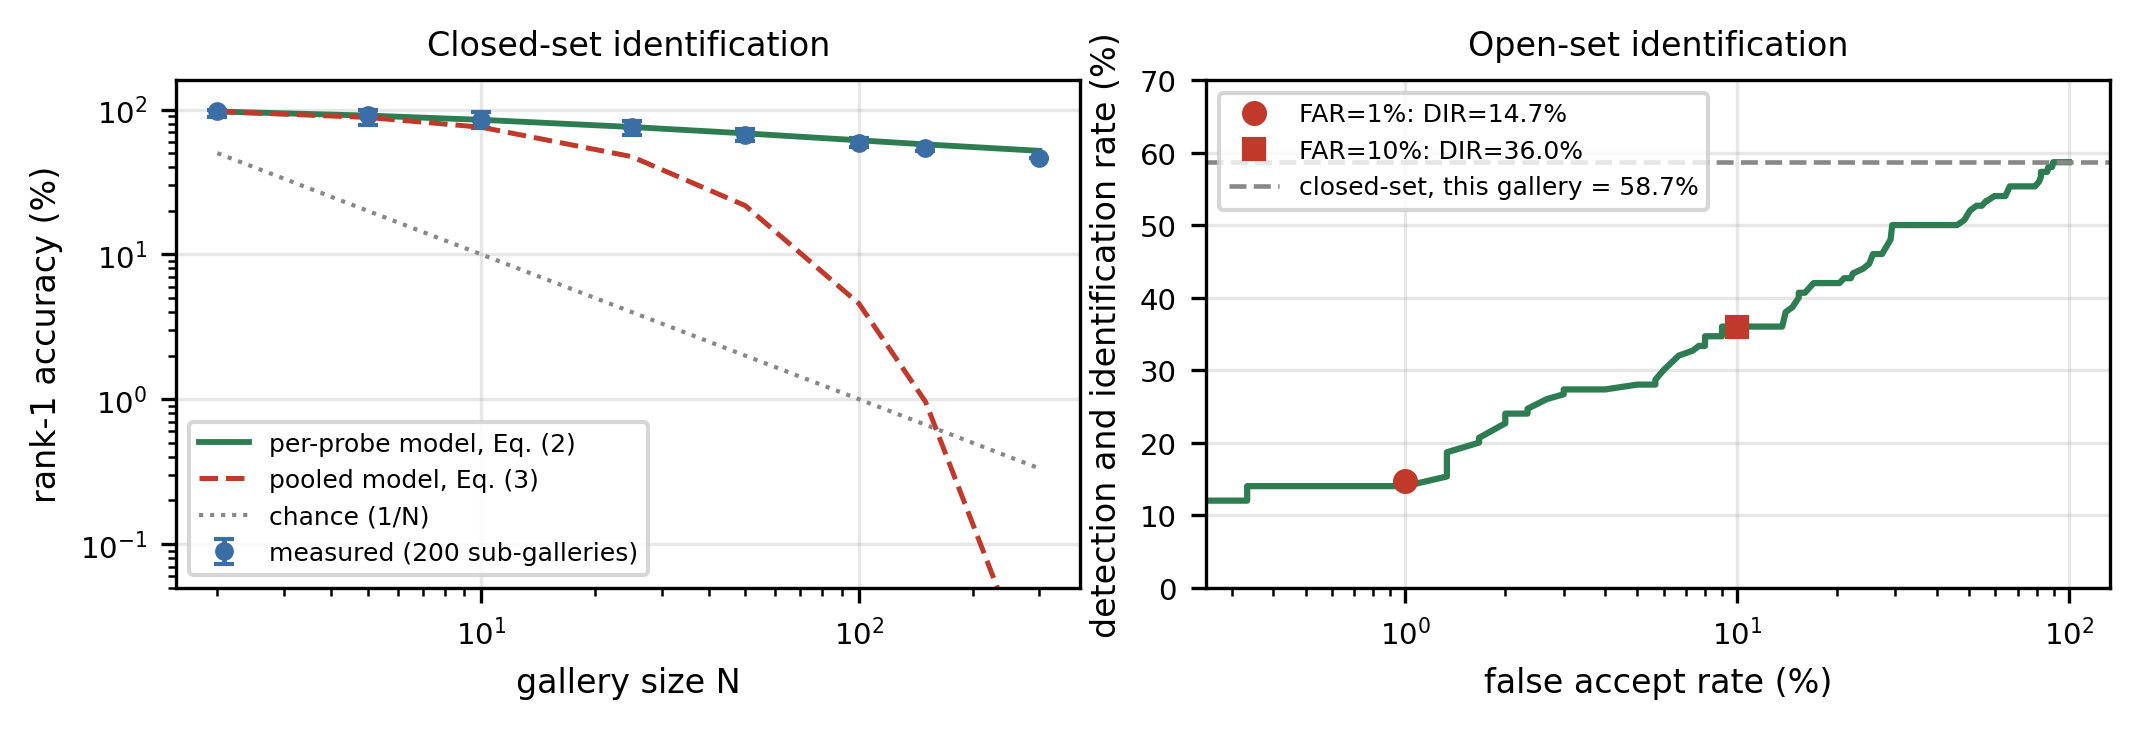
\includegraphics[width=\textwidth]{ieee_identification.png}
\caption{Left: measured closed-set rank-1 against gallery size, with both models
         overlaid. The logarithmic ordinate is needed to contain the collapse of
         Eq.~(\ref{eq:pool}), which compresses the measured points and
         Eq.~(\ref{eq:probe}) into the top of the axis; Table~\ref{tab:orderstats}
         is the better reference for the size of that residual. Right: open-set
         operating curve for the fixed $150$-identity gallery.}
\label{fig:ident}
\end{figure*}

\subsection{Open-Set Identification Performance}
\label{sec:openset}

Adding 300 people without reference photos in the database greatly reduced performance. For a fixed database of 150 people, the closed-set rank-1 accuracy was 58.7\%, but the Detection and Identification Rate (DIR) dropped to 14.7\% at a 1\% False Accept Rate (FAR) and 36.0\% at a 10\% FAR. Reaching the same 58.7\% closed-set accuracy would require a threshold of approximately $(\tau \approx 0.9)$, but at this threshold 94.7\% of unknown people would be incorrectly accepted. The reported closed-set accuracy refers only to this single fixed database of 150 people, not the average over the 200 randomly generated databases reported in Table ~\ref{tab:orderstats}.

Open-set identification is more difficult because two conditions must be met at the same time. First, the correct identity must be the closest match among the 149 other reference photos. Second, the matching distance must also be below a threshold that rejects unknown people. These two requirements work against each other, making open-set identification much more challenging. As a result, the practical open-set performance is much lower than both the closed-set identification and verification performance.

\subsection{Multi-Reference Photos}
\label{sec:multishot}
Improving the similarity between a person's reference photos and test image, rather than changing the matching method, should improve identification accuracy. To test this, each person's reference photo was replaced with the normalized average of \(k\) face embeddings, while keeping the database size and test images the same.

Table~\ref{tab:multishot} confirms this prediction. Averaging multiple reference photos also reduced the distances for incorrect matches, from 0.735 to 0.708, but it reduced the distance for the correct matches by a much larger amount, from 0.743 to 0.627. As a result, the margin changed from (-0.008) to (+0.081). This means the improvement came from more correct test images being identified successfully, rather than all embeddings simply becoming closer together. The method required no changes to the network, threshold, or matching rule. The single-reference-photo baseline was 52.0\% because this experiment used only the 610 people with at least four photos available.


\begin{table}[!t]
\caption{Effect of using multiple reference photos on closed-set identification accuracy and matching distances.}
\label{tab:multishot}
\centering
\begin{tabular}{ccccc}
\toprule
$k$ & Rank-1 & Genuine $d$ & $\mathbb{E}[\min d_{\text{imp}}]$ & Margin \\
\midrule
1 & 52.0\% & 0.743 & 0.735 & $-0.008$ \\
2 & 62.7\% & 0.666 & 0.715 & $+0.049$ \\
3 & \textbf{69.3\%} & \textbf{0.627} & 0.708 & $\mathbf{+0.081}$ \\
\bottomrule
\end{tabular}
\end{table}


%==============================================================================
\section{Discussion}
%==============================================================================

\subsection{Identification Failure Analysis}

Successful test images matched their correct reference photo with an average distance of 0.58, which was below the matching threshold, while unsuccessful test images had an average distance of 0.95, which was above the threshold. The rank of the correct identity was strongly correlated with the genuine matching distance, with a Spearman correlation of $(\rho = 0.88)$. The average distance to the five nearest incorrect identities showed almost no correlation with rank $((\rho = -0.03,; p = 0.56))$. After accounting for this, the correlation between genuine distance and rank increased to $(\rho = 0.93)$. This indicates that identification performance mainly depends on how close a test image is to its correct reference photo, not to nearby incorrect identities.

Consistent with this, the correct identity usually remains near the top. Using
$1$-indexed ranks, the median rank of the true identity is $2$, with top-$5$
accuracy $71.0\%$ and top-$25$ accuracy $88.7\%$ against rank-$1$ of $46.7\%$ on
the full $300$-identity pool.

\subsection{Comparison of Fixed Cropping and Face Detection}
\label{sec:detector}

Because a fixed crop cannot adjust to faces that are not centered, we replaced it with OpenCV's YuNet face detector, which crops the detected face automatically. The detector successfully detected every image, but performance decreased. Using evaluation mentioned earlier, the fixed crop achieved 87.3\% verification accuracy and 58.7\% rank-1 identification accuracy, while the detector achieved only 85.2\% verification accuracy and 42.0\% rank-1 identification accuracy.

It is to be noted that this comparison is not completely fair. The fixed crop was carefully tuned using a separate tuning set, while the detector crop was only roughly tuned using the same data on which it was evaluated. This suggests that because the lfw-deepfunneled images were already aligned, using another face detector could not improve the alignment and instead introduced small variations in the crop position. These variations reduced identification accuracy by 16.7\%, compared with only 2.1\% for verification. It is also to be noted that the results cannot be easily reproduced as mention in Section I.

\subsection{Limitations}
\label{sec:threats}

This projects faces several limitations. The crop settings were originally chosen before the tuning and test sets were created, so a small amount of bias may still remain even after validation. In addition, the tuning and test sets share 99 images, and differences between the shifted crop sizes are mostly due to measurement noise.

The ten-fold cross-validation used random splits of the 600 image pairs instead of LFW's predefined identity-disjoint folds. This means the same person could appear in both the threshold-selection and evaluation folds, which may slightly overestimate performance. We also evaluated only 600 of the 3,000 available image pairs because of computational limits, resulting in wider confidence intervals.

Finally,  LFW mainly contains well-lit, frontal face images, the reported results are likely better than what would be achieved in more challenging real-world conditions. We also did not perform a demographic analysis, so the reported overall accuracy may hide differences in performance across different groups~\cite{buolamwini2018gendershades}.

%==============================================================================
\section{Conclusion and Future Work}
%==============================================================================

The final model achieved 89.2\% verification accuracy, 58.7\% closed-set rank-1 accuracy on a database of (N = 150) people, and 14.7\% open-set Detection and Identification Rate (DIR) at a 1\% False Accept Rate (FAR). These differences are not due to limitations of the model but to the increasing difficulty of each task. As the database size grows, the closest incorrect match becomes more similar to the test image, making closed-set identification more challenging. Open-set identification is even more difficult because the model must correctly identify the person while also rejecting unknown people, leading to a further decrease in performance.

The study also found that preprocessing had a greater impact on performance than changes to the model architecture. In particular, the vertical position of the crop window was as important as its size, while differences between crop sizes were mostly due to measurement noise.

The failure analysis showed that most identification errors occurred when the distance between a person's test image and reference photo was large. Using multiple reference photos reduced this distance and improved identification accuracy by 17.3\% without changing the model architecture. We also suggest that improved face alignment and newer models trained with angular-margin losses, such as ArcFace, could further improve performance.

\section{Disclaimer}
This paper was proofread with the assistance of an AI language tool for grammar and spelling. All ideas, analysis, and conclusions are the authors' own.

\balance
\begin{thebibliography}{99}

\bibitem{schroff2015facenet}
F.~Schroff, D.~Kalenichenko, and J.~Philbin, ``FaceNet: A unified embedding for
face recognition and clustering,'' in \emph{Proc. IEEE CVPR}, 2015, pp.\ 815--823.

\bibitem{taigman2014deepface}
Y.~Taigman, M.~Yang, M.~Ranzato, and L.~Wolf, ``DeepFace: Closing the gap to
human-level performance in face verification,'' in \emph{Proc. IEEE CVPR}, 2014,
pp.\ 1701--1708.

\bibitem{amos2016openface}
B.~Amos, B.~Ludwiczuk, and M.~Satyanarayanan, ``OpenFace: A general-purpose face
recognition library with mobile applications,'' Carnegie Mellon Univ.,
Tech. Rep. CMU-CS-16-118, 2016.

\bibitem{huang2007lfw}
G.~B.~Huang, M.~Ramesh, T.~Berg, and E.~Learned-Miller, ``Labeled faces in the
wild: A database for studying face recognition in unconstrained environments,''
Univ. of Massachusetts, Amherst, Tech. Rep. 07-49, Oct. 2007.

\bibitem{szegedy2015going}
C.~Szegedy, W.~Liu, Y.~Jia, P.~Sermanet, S.~Reed, D.~Anguelov, D.~Erhan,
V.~Vanhoucke, and A.~Rabinovich, ``Going deeper with convolutions,'' in
\emph{Proc. IEEE CVPR}, 2015, pp.\ 1--9.

\bibitem{kemelmacher2016megaface}
I.~Kemelmacher-Shlizerman, S.~Seitz, D.~Miller, and E.~Brossard, ``The MegaFace
benchmark: 1 million faces for recognition at scale,'' in \emph{Proc. IEEE CVPR},
2016, pp.\ 4873--4882.

\bibitem{klare2015ijba}
B.~F.~Klare, B.~Klein, E.~Taborsky, A.~Blanton, J.~Cheney, K.~Allen, P.~Grother,
A.~Mah, and A.~K.~Jain, ``Pushing the frontiers of unconstrained face detection and
recognition: IARPA Janus Benchmark A,'' in \emph{Proc. IEEE CVPR}, 2015,
pp.\ 1931--1939.

\bibitem{radovanovic2010hubs}
M.~Radovanovi\'{c}, A.~Nanopoulos, and M.~Ivanovi\'{c}, ``Hubs in space: Popular
nearest neighbors in high-dimensional data,'' \emph{J. Mach. Learn. Res.}, vol.~11,
pp.\ 2487--2531, 2010.

\bibitem{wang2018cosface}
H.~Wang, Y.~Wang, Z.~Zhou, X.~Ji, D.~Gong, J.~Zhou, Z.~Li, and W.~Liu, ``CosFace:
Large margin cosine loss for deep face recognition,'' in \emph{Proc. IEEE CVPR},
2018, pp.\ 5265--5274.

\bibitem{deng2019arcface}
J.~Deng, J.~Guo, N.~Xue, and S.~Zafeiriou, ``ArcFace: Additive angular margin loss
for deep face recognition,'' in \emph{Proc. IEEE CVPR}, 2019, pp.\ 4690--4699.

\bibitem{buolamwini2018gendershades}
J.~Buolamwini and T.~Gebru, ``Gender shades: Intersectional accuracy disparities in
commercial gender classification,'' in \emph{Proc. Conf. Fairness, Accountability
and Transparency}, 2018, pp.\ 77--91.

\end{thebibliography}


\end{document}
